%%%%%%%%%%%%%%%%%%%%%%%%%%%%%%%%%
%
%       EXERCÍCIO
%
%%%%%%%%%%%%%%%%%%%%%%%%%%%%%%%%%

\definevalorquestao

\begin{exercicioBanco}[\valorquestao]
A função real \(f\) definida por \(f(x) = a \cdot 3^x + b\), sendo \(a\) e \(b\) constantes reais, está graficamente representada abaixo.

\begin{center}
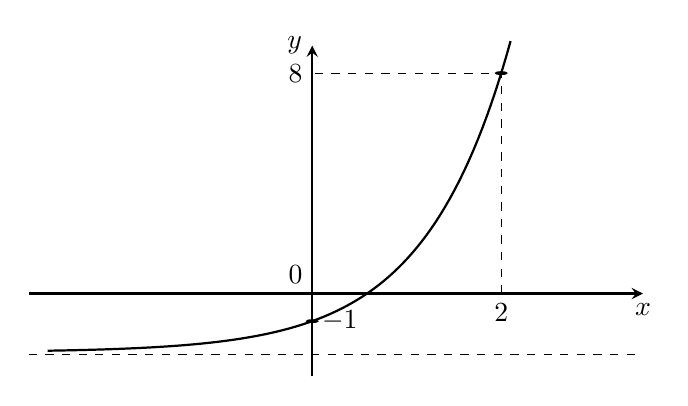
\begin{tikzpicture}[xscale=1.2, yscale=0.35, >=stealth]
    % Eixos cartesiano
    \draw[->, thick] (-3,0) -- (3.5,0) node[below] {$x$};
    \draw[->, thick] (0,-3) -- (0,9) node[left] {$y$};
    \node[above left] at (0,0) {$0$};
    
    % Assíntota horizontal
    \draw[dashed] (-3,-2.2) -- (3.5,-2.2);
    
    % Gráfico da função f(x) = (9/8)*3^x - 17/8
    \draw[thick, domain=-2.8:2.1, samples=100] plot (\x, {1.125*3^(\x) - 2.125});
    
    % Marcadores dos pontos (0, -1) e (2, 8)
    \draw[dashed] (2,0) -- (2,8) -- (0,8);
    \node[below] at (2,0) {$2$};
    \node[left] at (0,8) {$8$};
    \node[right] at (0,-1) {$-1$};
    
    \fill (0,-1) circle (2pt);
    \fill (2,8) circle (2pt);
\end{tikzpicture}
\end{center}

Pode-se afirmar que o produto \(a \cdot b\) pertence ao intervalo real:

% Define as alternativas
\newcommand{\alternativas}{%
    \begin{center}
        \begin{tabularx}{\textwidth}{XXXXX}
            (a) \([-4,-1]\). &
            (b) \([-1,2[\). &
            (c) \([2,5[\). &
            (d) \([5,8]\). &
            (e) \([8,11]\).
        \end{tabularx}
    \end{center}
}

% Define a resposta correta
\newcommand{\resposta}{A}

% Lógica condicional para exibição
\ifdefstring{\atividade}{lista}{%
    \alternativas
    \vspace{0.5em}
    
    \noindent\textbf{Resposta:} letra \textbf{\resposta}.
}{%
    \ifdefstring{\modo}{objetivo}{%
        \alternativas
    }{%
        % modo = discursiva → não mostra alternativas
    }
}
\end{exercicioBanco}

